\documentclass[11pt]{article}
\usepackage[margin=1in]{geometry}
\usepackage{amsmath,amssymb}
\usepackage{booktabs}
\usepackage{graphicx}
\usepackage{longtable}
\usepackage{xcolor}
\usepackage{hyperref}
\hypersetup{colorlinks=true,linkcolor=blue,urlcolor=blue}
\graphicspath{{../figures/}}

\title{DBACT sampled discrete-dissipation: advisor delivery report\\
\large Static uniform-offset theorem\_mode, $N=16$, nine cases}
\author{Branch \texttt{feat/sampled-theorem-mode} on frozen baseline \texttt{98ba28e} (not merged)}
\date{2026-09-11}

\newcommand{\gstar}{g^\star}
\newcommand{\Hstar}{H^\star}
\newcommand{\umax}{u_{\max}}

\begin{document}
\maketitle

\begin{abstract}
We repaired the sample-and-hold execution interface of the sampled
\texttt{theorem\_mode} controller and derived a discrete truncated-coverage
inequality with a mass-weighted command-energy indicator $J$. This report
delivers the honest verdict: the post-hoc numbers are informative and the
conditional dissipation structure is sound, but there is \emph{no} a priori
centroid-error bound that turns the new estimate into a certified quantitative
improvement over a model-free geometric ceiling, the $N=16$ Hessian / local
stability question remains open, and the static-oracle runs are theory
baselines --- \textbf{not} a certificate for unknown-object transport. All nine
cases (L-shape, rectangle, C-channel $\times$ seeds 2/5/8) complete 30\,s with
zero aborts; the C-channel seed~5 full-horizon $J$ bound is explicitly
\emph{inapplicable}. The corrected derivation is in \S\ref{sec:derivation}.
\end{abstract}

\section{One-line verdict}
Original coarse Theorem~1 bound: \emph{no quantitative value} (it loses to a
model-free geometry ceiling a priori). New discrete results: \emph{conditional
dissipation} plus \emph{post-hoc explanatory value}. \textbf{No} a priori
guarantee beating geometry. Static oracle $\neq$ unknown-object transport
proved.

\section{Point-by-point responses}

\paragraph{A5 and hard switching.} Assumption~5 (locally Lipschitz
continuous-time feedback) is still incompatible with the endpoint-grid CVT path:
hard disk / Voronoi membership on a finite $20\times20$ lattice produces finite
centroid jumps under arbitrarily small site moves. The present branch does
\emph{not} claim the production CVT satisfies A5; it isolates a different
interface: static sample-and-hold cover with wall rows, no position clipping,
abort-on-illegal, and a Lipschitz-certified object-hold clearance.

\paragraph{Why the original Theorem~1 bound lacks quantitative value.} Under the
default static parameters the printed asymptotic formula evaluates to
$\approx 1.90\times10^{4}$ for the gradient-squared residual, while a direct
total-mass geometric ceiling is $\approx 8.99$, and measured 30\,s time averages
are $\approx 0.011$--$0.013$. The formula is therefore worse than a model-free
geometry bound by $\sim 2\times10^{3}$ and orders of magnitude above
observation. Replacing the printed number by $\min(\text{formula},\text{geometry})$
would hide the missing information, not create theory.

\paragraph{What the new discrete results establish.}
\begin{enumerate}
\item \textbf{Proved (fixed $\phi^\star$).} The frozen truncated-partition
majorant (Lemma~A) gives the discrete inequality~\eqref{eq:discrete-ineq}
without assuming dissipation.
\item \textbf{Proved ($a=2/k_c-\Delta>0$).} The exact-centroid / unsaturated
pairing structure for a discrete decrease along centroid-aligned commands
(Theorem~B).
\item \textbf{Conditional.} Projection comparison against $0$ holds only on
steps in $\mathcal{K}_0$ (final QP set with the $\rho$ margin); this is not
promoted from ``true on some L-runs'' to a global fact --- the C-channel seed~5
already exhibits six agent-steps with $0\notin F_\rho$.
\item \textbf{Post-hoc.} With mass-weighted $J_k,E_k$, the finite-horizon form
$(\star)$ matches L-shape measurements when $\bar E$ is taken from the
trajectory.
\item \textbf{$J$ is not the gradient residual.} Vanishing command speed does
not imply vanishing $\gstar$.
\end{enumerate}

\paragraph{$N=16$ Hessian.} No Hessian / curvature / invariant-neighborhood
certificate was computed or claimed. This remains an open item, out of scope for
this round by design.

\paragraph{A3 --- same Gaussian kernel.} The offset density and the continuous
observer share the same unnormalized Gaussian edge kernel $K_\sigma$ with a
single $\sigma$ and nonnegative weights; the manuscript should state this
interface explicitly so Lemma-type constants have a clear domain.

\section{Quantitative summary (static oracle, $N=16$, 30\,s)}

\begin{center}
\begin{tabular}{lccc}
\toprule
Block & Theorem-1 / analytic & Geometric & Measured \\
\midrule
$\|\gstar\|^2$ avg & $\approx1.90\times10^4$ (\emph{not a cert.}) & $\approx8.99$ & $\approx0.011$--$0.013$ (L) \\
Mass-weighted $J$ & post-hoc $(\star)\approx0.025$--$0.034$ & $M\umax^2\approx0.18$--$0.23$ (preferred) & $\bar J\approx0.009$--$0.012$ \\
Centroid $E$ & --- & diameter $4R^2M\approx4.80$ (loose) & $\bar E\sim10^{-4}$ (\emph{post-hoc}) \\
\bottomrule
\end{tabular}
\end{center}

\noindent\textbf{A priori error bound sufficient to beat geometry?} \textbf{No.}
Against the preferred geometric $J$ ceiling $M\umax^2$, one needs $\bar E\le
E^\star$; the only model-only bound is the resolution-independent diameter bound
$\approx4.8>E^\star$, which does not control grid/oracle centroid error. We
refuse to treat trajectory $\max E$ as a uniform prior. Post-hoc, measured
$\bar E\sim10^{-4}$ makes $(\star)$ look useful --- explanatory, not certified.

\subsection{Nine-case table}
All nine cases complete 30\,s with zero aborts. The C-channel seed~5 records six
zero-input-with-$\rho$ failures (frames 241--246, agent~14) and is the only case
with an \emph{inapplicable} full-horizon $J$ bound. The primary geometric $J$
ceiling is $M_{\mathrm{tot}}\umax^2$ (\emph{not} $N m_+\umax^2$).

\begingroup
\small
\begin{longtable}{llccccc}
\toprule
shape & seed & full-horizon & $H_0$ & $\bar J$ & post-hoc $J$ bd. & $M\umax^2$ \\
\midrule
\endhead
l\_shape & 2 & yes & 0.9754 & 0.01108 & 0.03006 & 0.2295 \\
l\_shape & 5 & yes & 0.9555 & 0.01071 & 0.02945 & 0.2295 \\
l\_shape & 8 & yes & 1.0297 & 0.01152 & 0.03169 & 0.2295 \\
rectangle & 2 & yes & 0.8140 & 0.00894 & 0.02507 & 0.1803 \\
rectangle & 5 & yes & 0.8262 & 0.00910 & 0.02551 & 0.1803 \\
rectangle & 8 & yes & 0.8495 & 0.00930 & 0.02618 & 0.1803 \\
c\_shape & 2 & yes & 1.0789 & 0.01201 & 0.03330 & 0.2295 \\
c\_shape & 5 & \textbf{no} & 1.0884 & 0.01234$^{\dagger}$ & inapplicable & 0.2295 \\
c\_shape & 8 & yes & 1.1109 & 0.01251 & 0.03432 & 0.2295 \\
\bottomrule
\end{longtable}
\endgroup
\noindent{\footnotesize $^{\dagger}$ descriptive statistic tagged
\texttt{not\_covered\_by\_theorem}; the post-hoc bound is not applied because
$\mathcal{K}_0\neq[0,K)$. Exact machine values are in
\texttt{nine\_case\_summary.json} and \texttt{nine\_case\_comparison.csv};
$M\umax^2$ values are recomputed offline from
\texttt{observer.total\_mass(vertices)}.}

\paragraph{Three-command check (fixed).} Each stage uses its own hypothetical
next pose $P+\Delta u$; on refinement $H$, $g$ and $m$ are all taken from the
same fine observer. Refined max slacks stay $O(10^{-6})$--$O(10^{-7})$:
numerical consistency at quadrature tolerance, \textbf{not} a strict numerical
certificate (\texttt{no\_rigorous\_quadrature\_error\_bound}). Per-case values
are in \texttt{three\_command\_hyp/}.

\section{Figures}
Discrete-average lines are the horizontal dashes; C-channel seed~5 condition
failures are shaded. The discrete average $(1/K)\sum_k$ and the trapezoidal
continuous-time approximation differ by $O(\Delta/T)$ (both reported in
\texttt{j\_bound/*.json}); the discrete mean is primary.

\begin{figure}[htbp]\centering
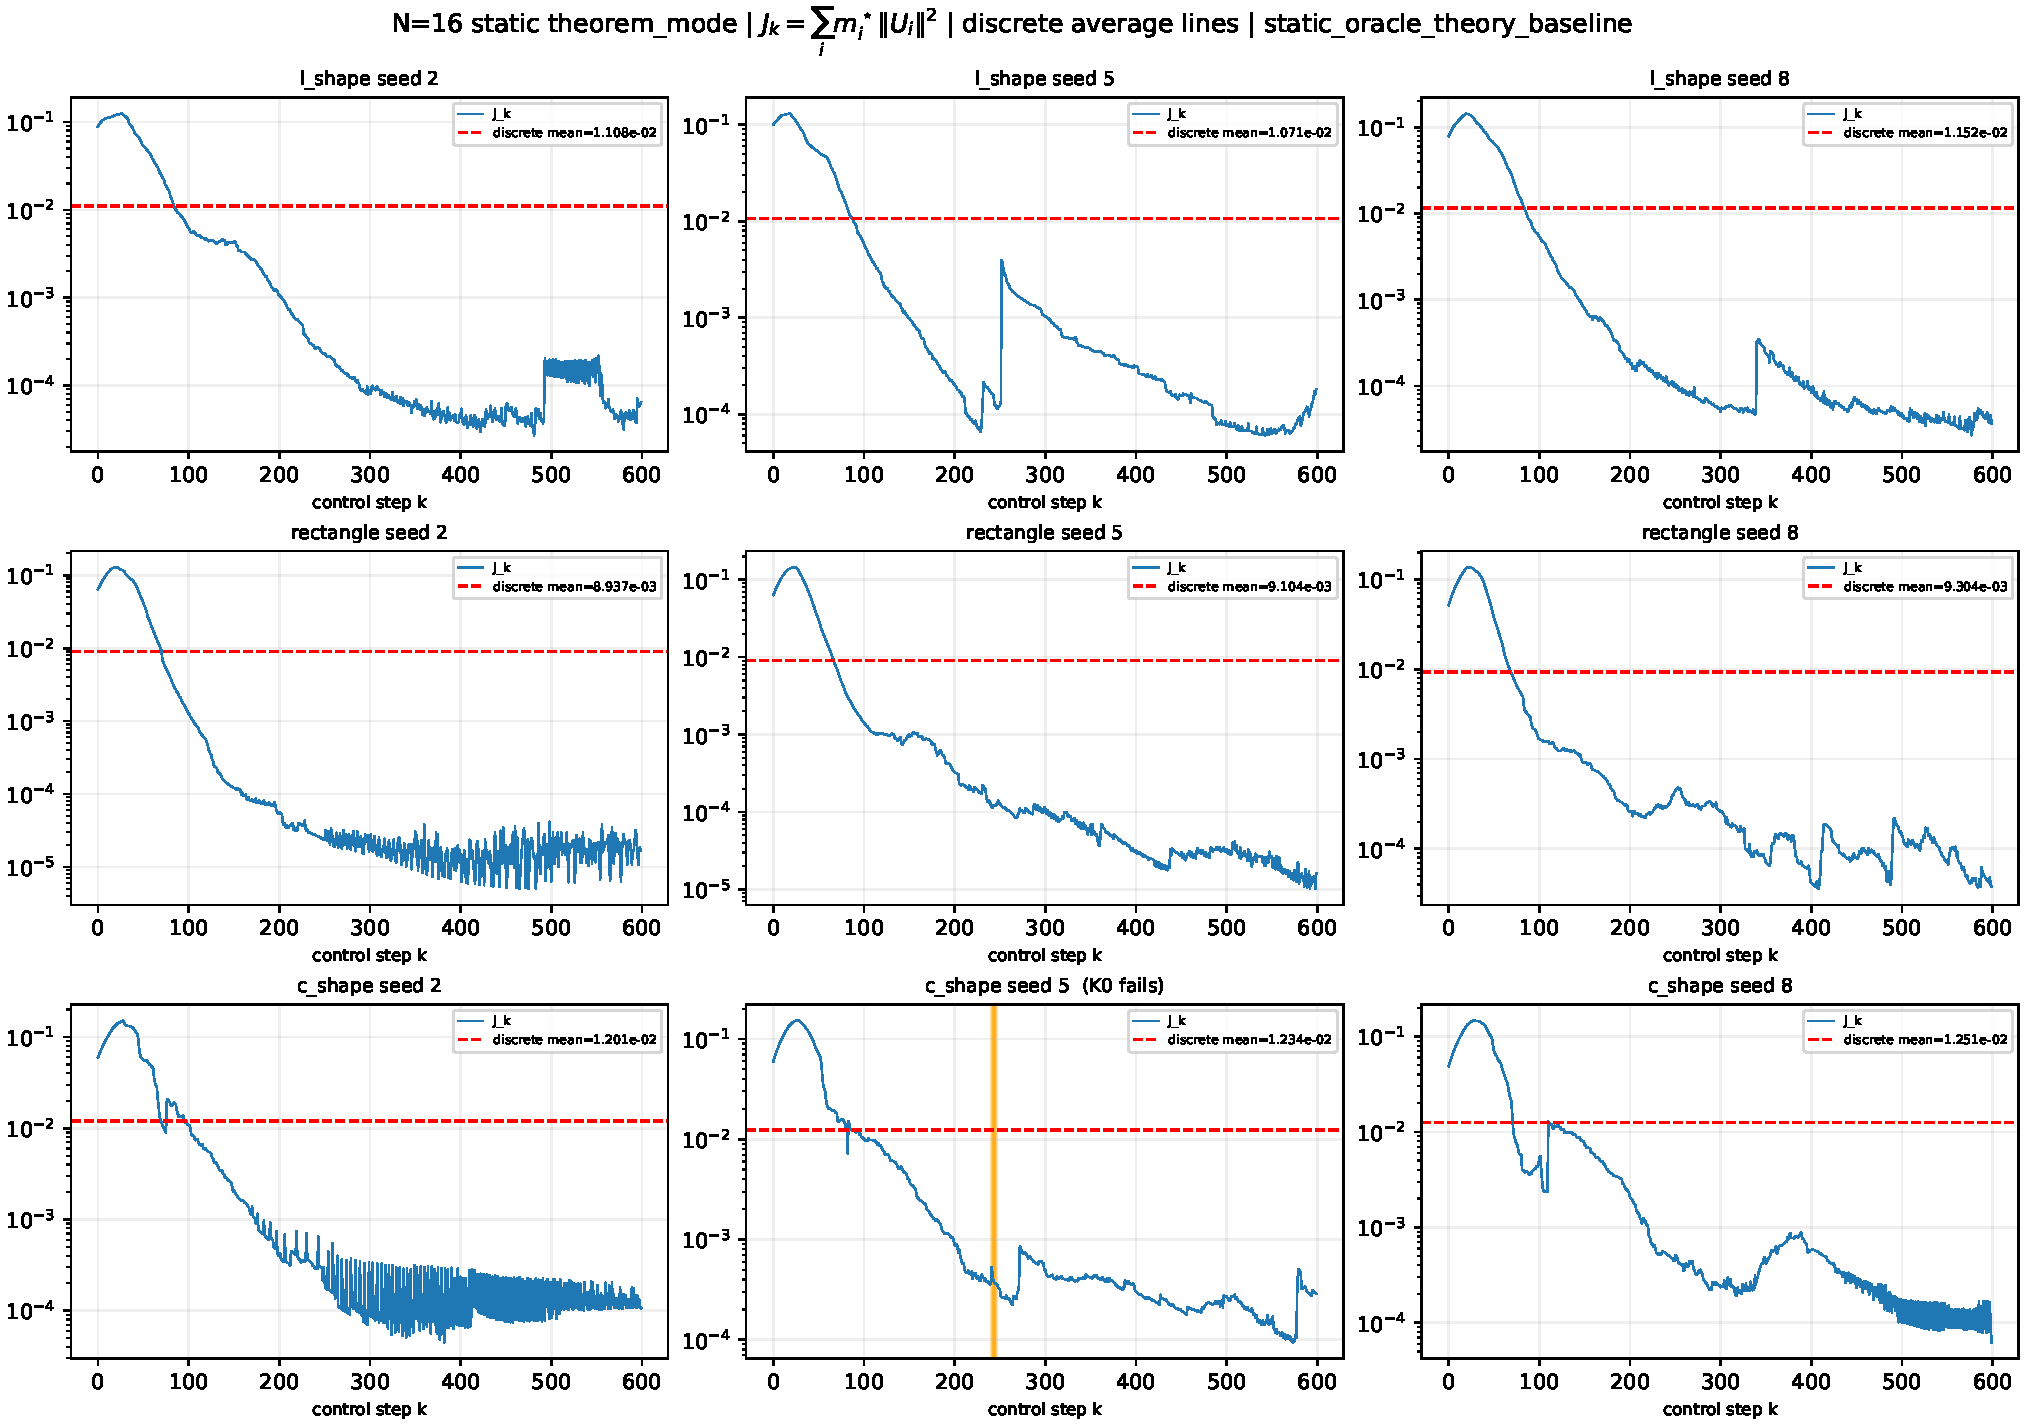
\includegraphics[width=0.9\textwidth]{nine_case_J.pdf}
\caption{$J_k=\sum_i m_i^\star\|U_i\|^2$ per case with discrete-average lines.}
\end{figure}

\begin{figure}[htbp]\centering
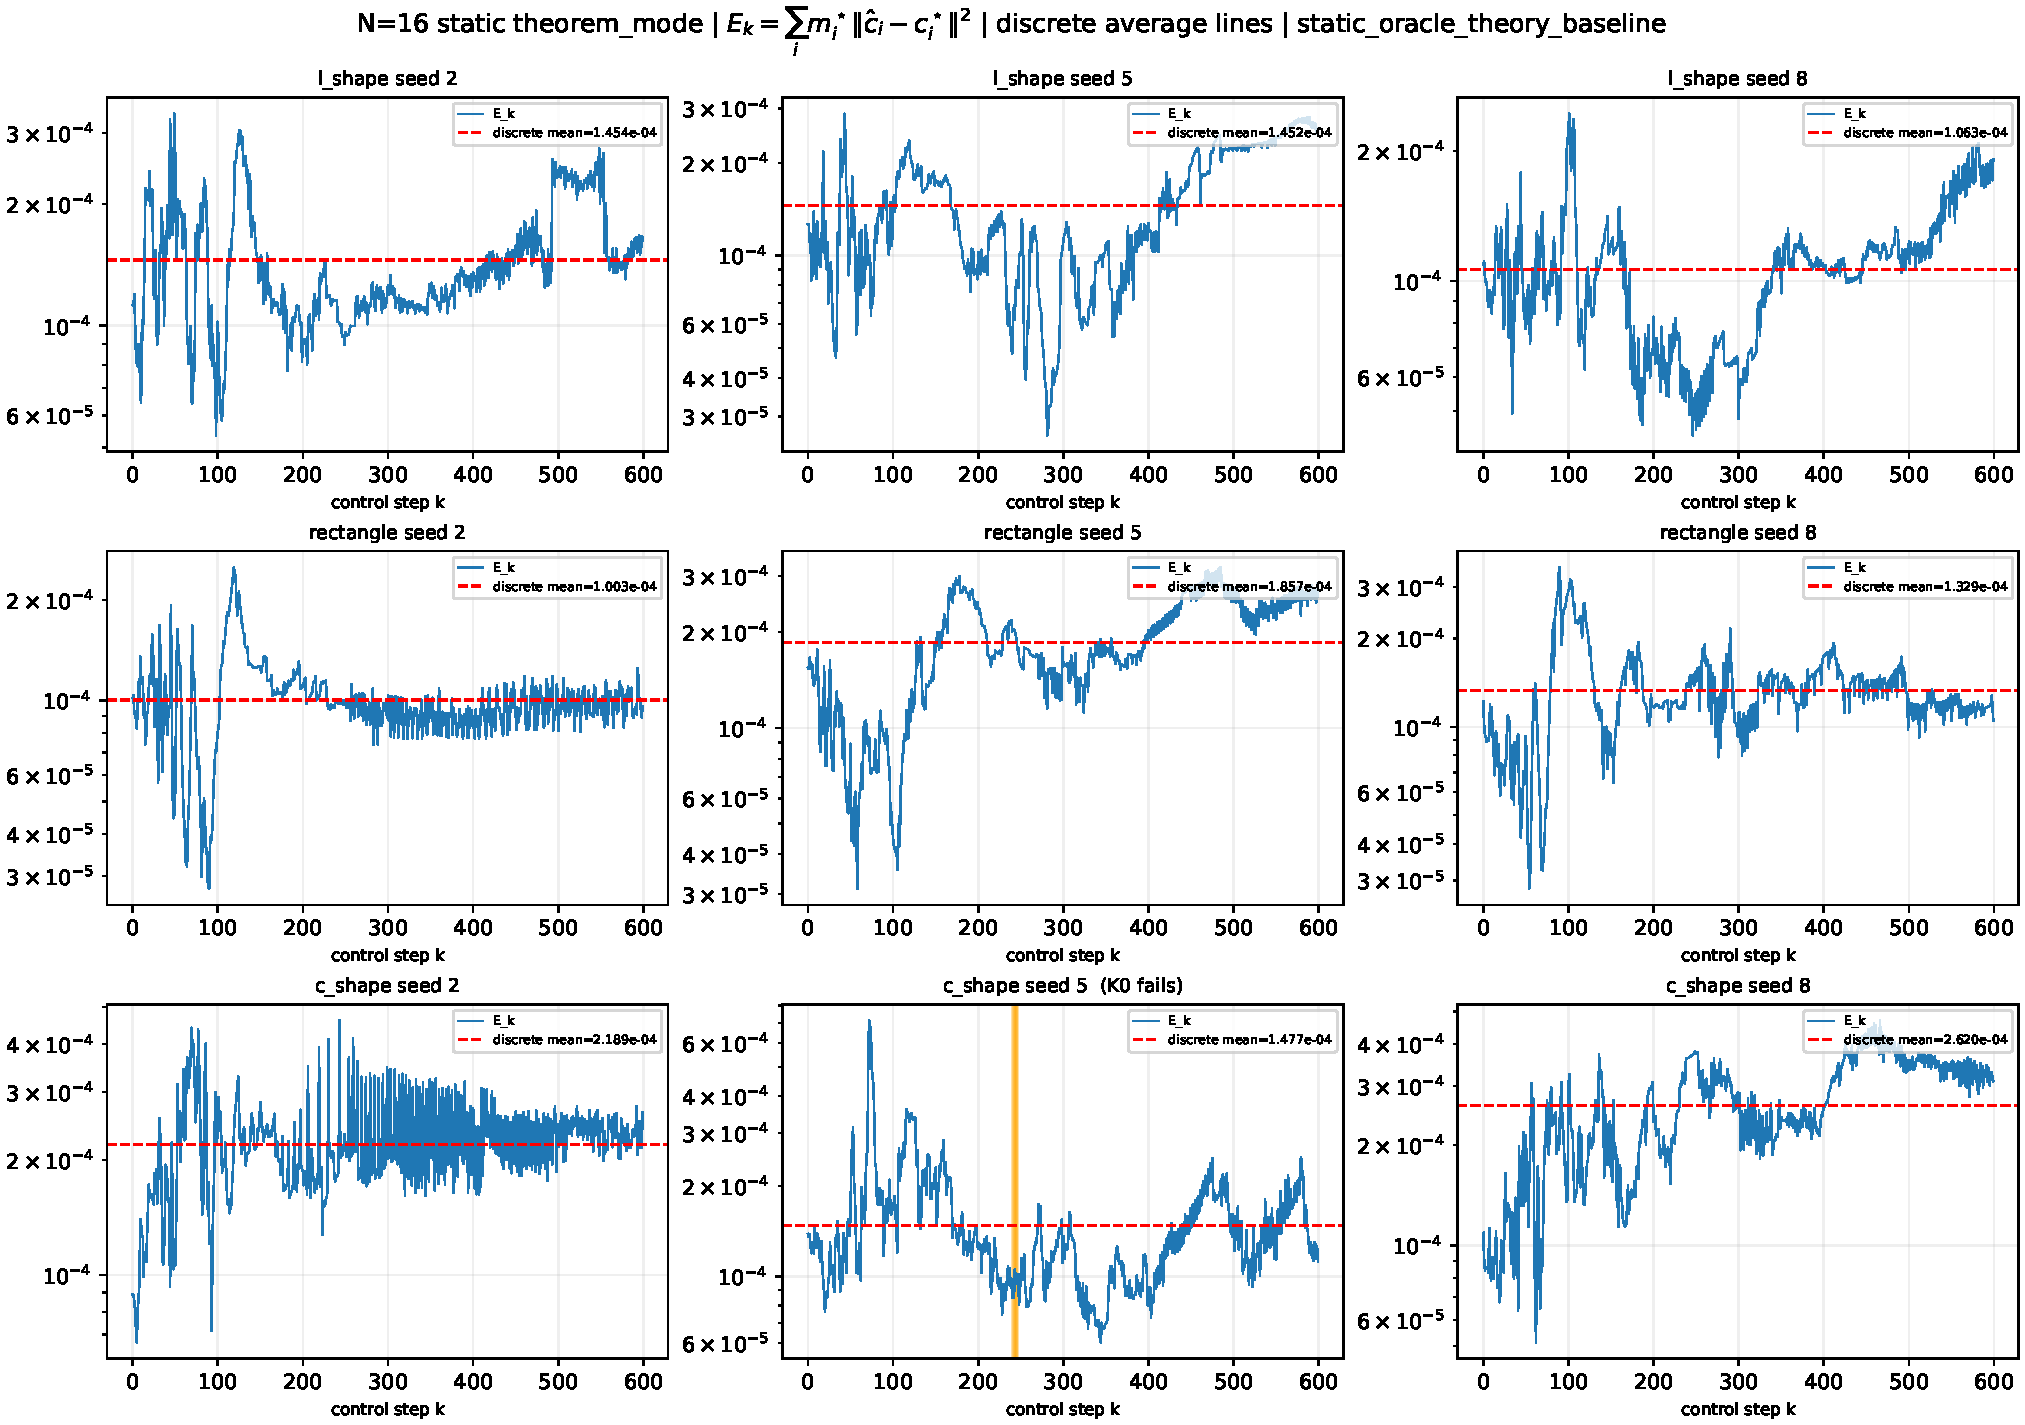
\includegraphics[width=0.9\textwidth]{nine_case_E.pdf}
\caption{$E_k=\sum_i m_i^\star\|\hat c_i-c_i^\star\|^2$ (post-hoc) per case.}
\end{figure}

\begin{figure}[htbp]\centering
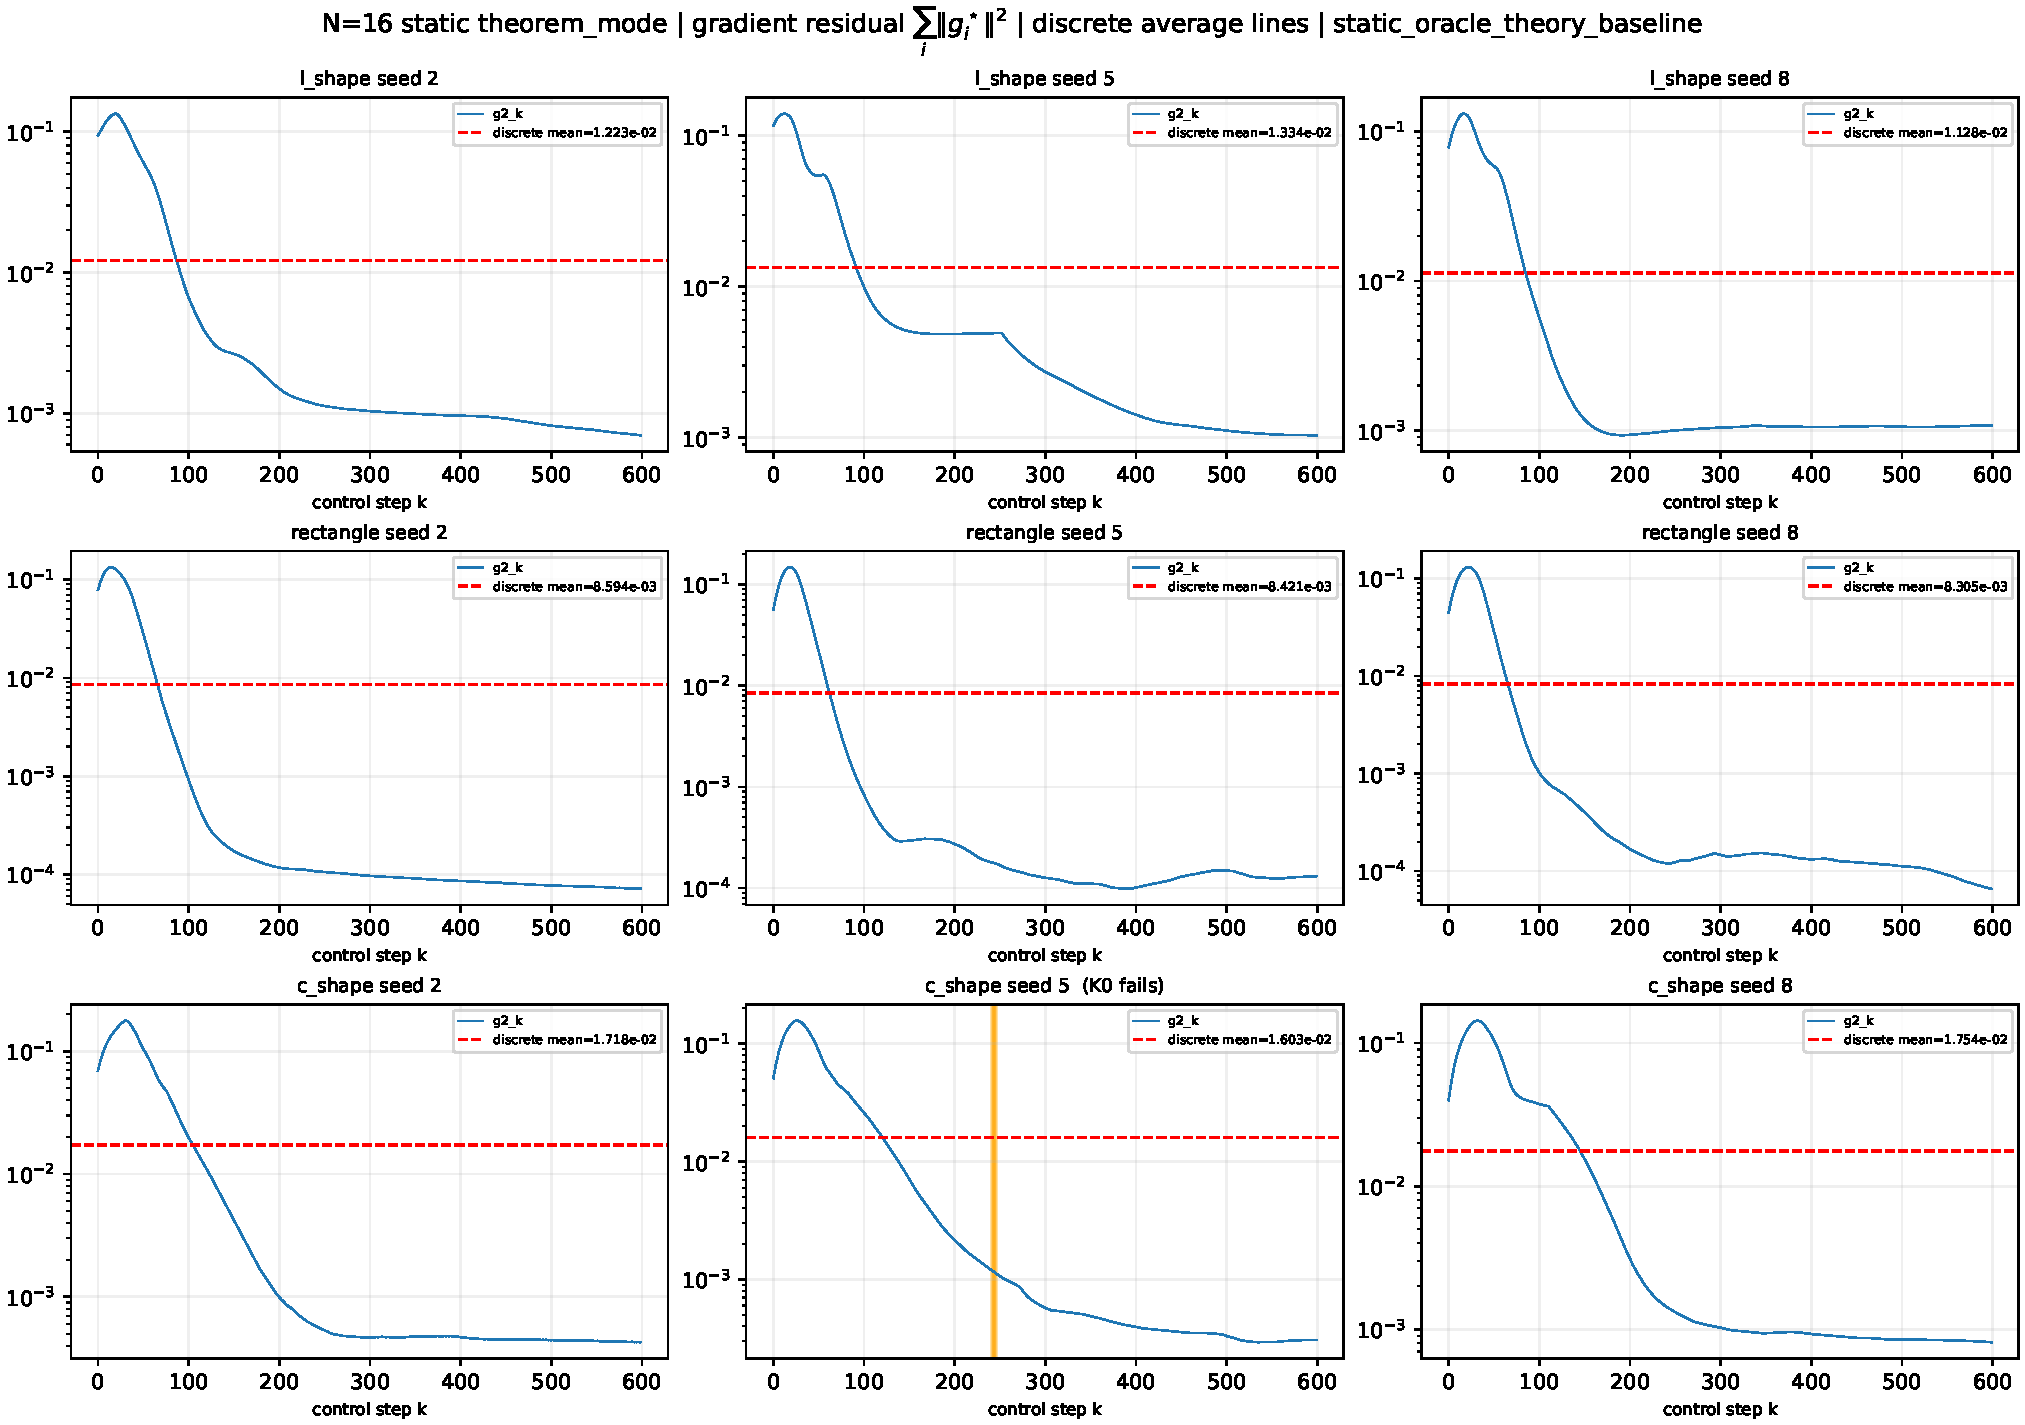
\includegraphics[width=0.9\textwidth]{nine_case_grad_residual.pdf}
\caption{Gradient residual $\sum_i\|\gstar_i\|^2$ per case (the original
paper indicator; distinct from $J$).}
\end{figure}

\begin{figure}[htbp]\centering
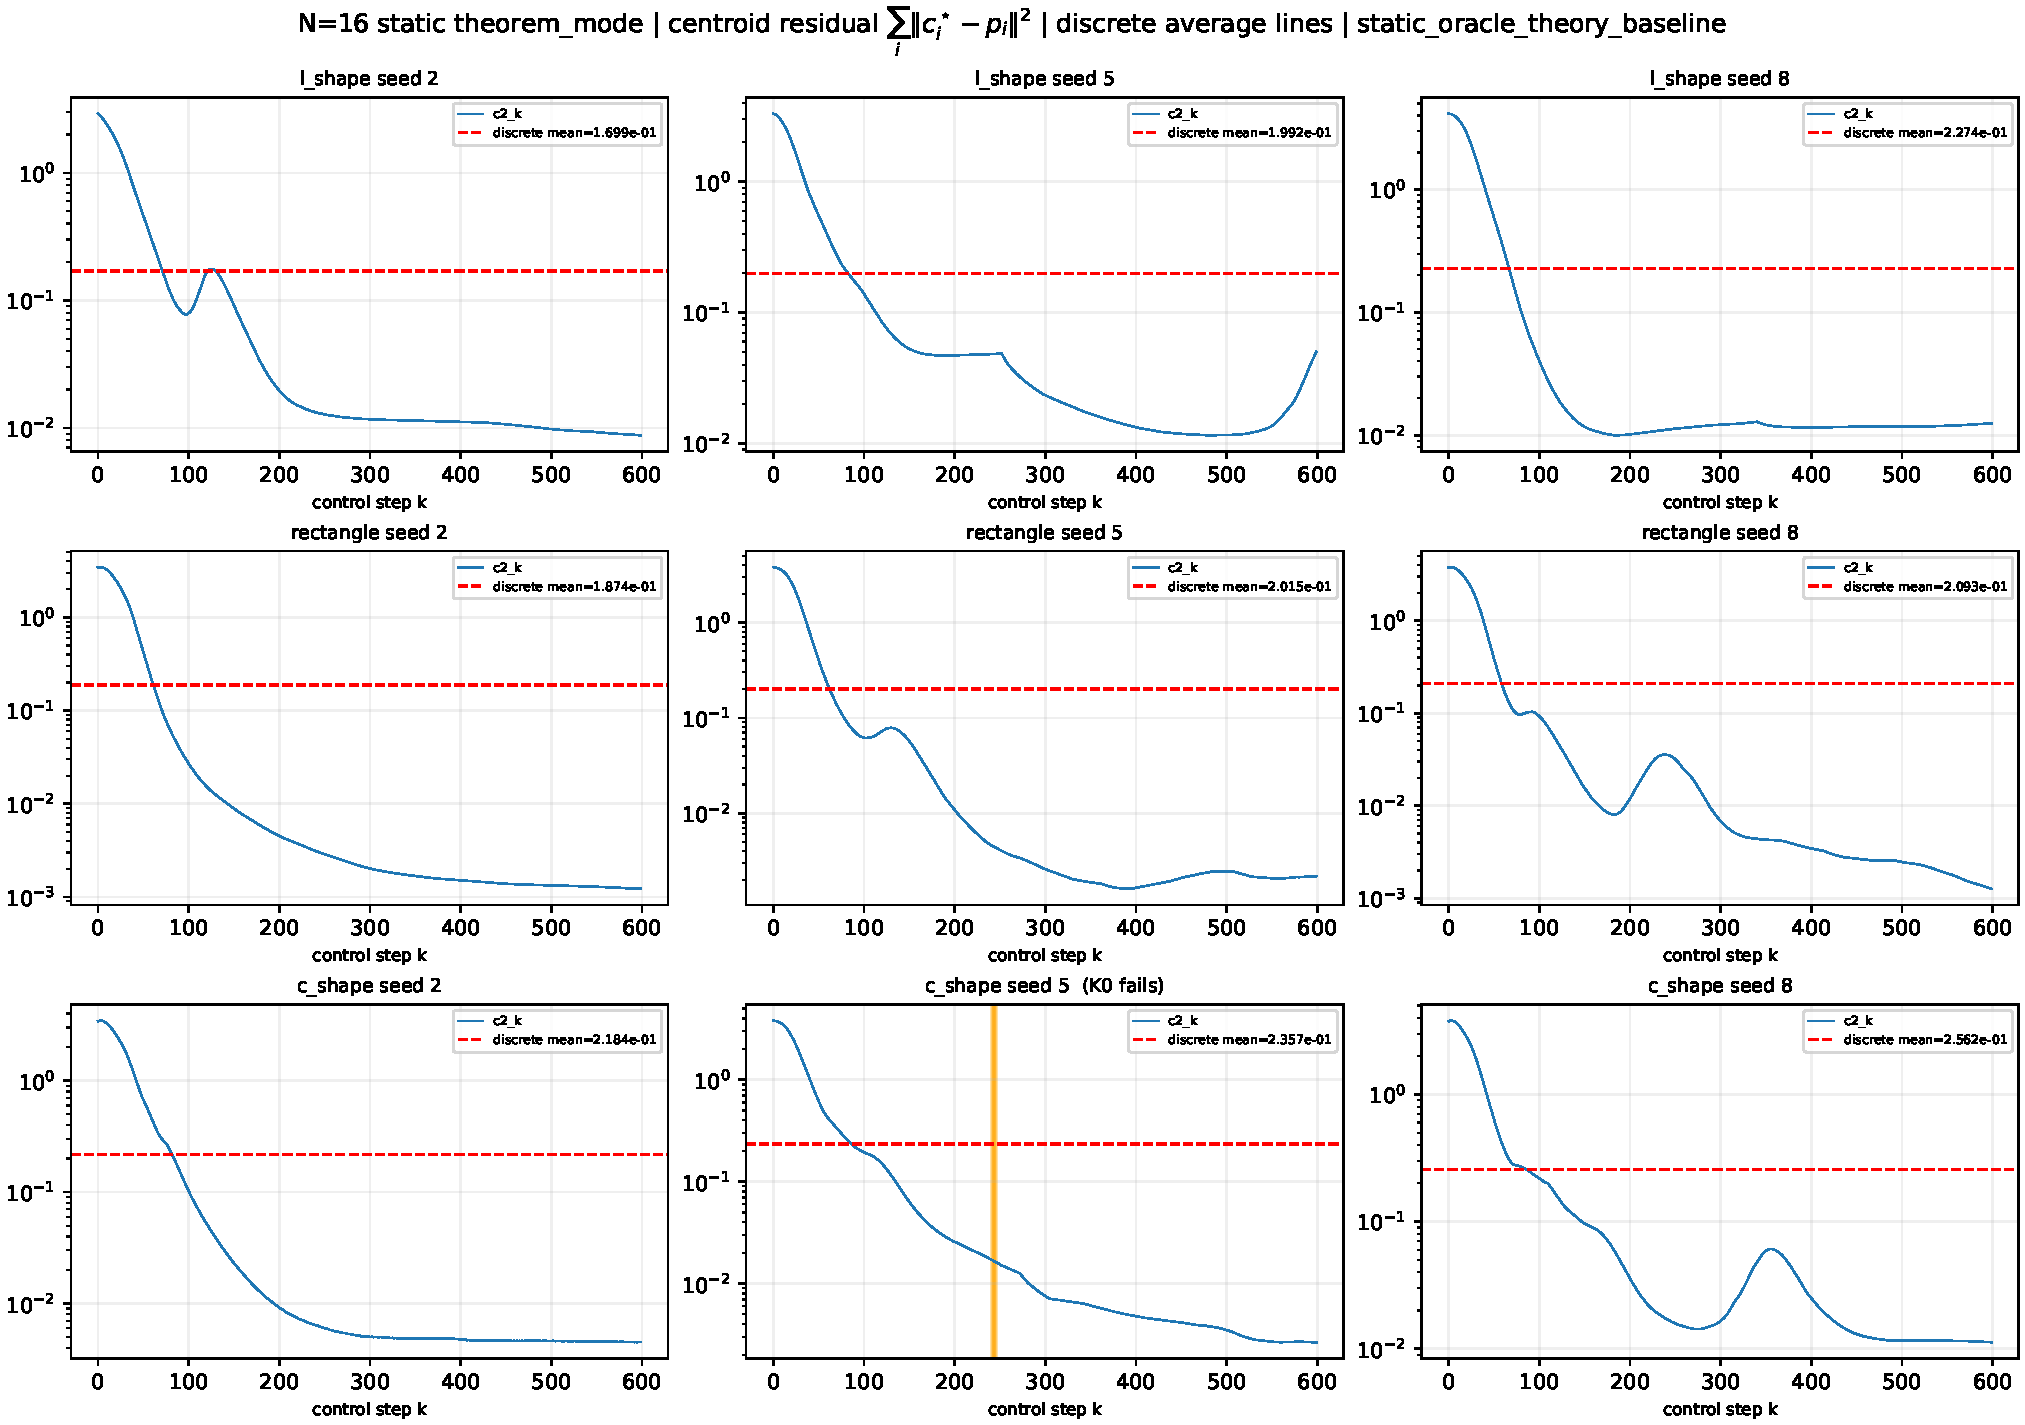
\includegraphics[width=0.9\textwidth]{nine_case_centroid_residual.pdf}
\caption{Centroid residual $\sum_i\|c_i^\star-p_i\|^2$ per case.}
\end{figure}

\section{Suggested paper revisions}
\begin{enumerate}
\item Split interfaces: continuous A5-style claims vs.\ sampled hold + abort.
\item Retire the coarse Theorem~1 formula as the main quantitative claim; report
geometry alongside any analytic bound.
\item Introduce the discrete candidate as Theorem~1$'$ (sampled, fixed density)
with Lemma~A, $a>0$, and explicit $\mathcal{K}_0$ conditioning.
\item Keep $e_i=\hat c_i-c_i^\star$ and mass weights visible; separate $J$ from
$\|\gstar\|^2$; mark post-hoc substitutions.
\item Write A3 with a single $K_\sigma$.
\item State the $N=16$ Hessian as open.
\item Safety subsection: wall rows + no clip + abort; object hold via a Lipschitz
clearance lower bound, not QP feasibility alone.
\end{enumerate}

\section{Open problems}
\begin{enumerate}
\item A resolution-dependent a priori bound on $\|\hat c_{\mathrm{grid}}-c^\star\|$
tight enough that $(\star)$ beats $M\umax^2$ without trajectory $E$: \emph{not
available}.
\item Closing dissipation for final QP commands outside $\mathcal{K}_0$ without
deleting $\rho$.
\item $N=16$ Hessian / conditional local-stability certificate.
\item Extending beyond static oracle to unknown moving objects with map-error
bounds.
\item Replacing hard-grid CVT if a continuous A5 statement is still desired.
\end{enumerate}

% ---- Corrected derivation appendix ----
\appendix
% Derivation appendix: sampled discrete-dissipation candidate.
% Included from main.tex (no preamble here).
\section{Corrected derivation (sampled, fixed density)}
\label{sec:derivation}

Throughout, sites are $P=(p_1,\dots,p_N)$ and commands $u=(u_1,\dots,u_N)$; the
uncovered region is $\mathcal{U}(P)=D\setminus\bigcup_i\Omega_i(P)$ (we never
reuse the symbol $U$ for both the command and the uncovered set). The reference
density $\phi^\star\ge0$ is \emph{fixed} and the execution is sample-and-hold,
$P_{k+1}=P_k+\Delta u_k$.

\paragraph{Status labels.}
\emph{Proved} = mathematical under the stated hypotheses;
\emph{Conditional} = proved only on execution steps where named conditions hold,
never inferred globally from finite runs;
\emph{Post-hoc numerical} = trajectory / quadrature evaluation;
\emph{Strict numerical certificate} = \textbf{not claimed} here (refined slacks
remain $O(10^{-6})$--$O(10^{-7})$, quadrature-limited).

\subsection{Lemma A (frozen truncated-partition majorant)}
Fix $\phi^\star$ on $D$ and radius $R>0$. With truncated cells
$\Omega_i(P)=V_i(P)\cap B(p_i,R)$ and
\[
H^\star(P)=\sum_i\int_{\Omega_i(P)}\|q-p_i\|^2\phi^\star\,dq
+R^2\int_{\mathcal{U}(P)}\phi^\star\,dq ,
\]
define per-cell mass, centroid and (observer-compatible) gradient
\[
m_i^\star=\int_{\Omega_i}\phi^\star,\quad
c_i^\star=\tfrac1{m_i^\star}\int_{\Omega_i}q\,\phi^\star,\quad
g_i^\star=2\,m_i^\star\,(p_i-c_i^\star).
\]
At step $k$ freeze the partition $\Omega_{i,k}=\Omega_i(P_k)$,
$\mathcal{U}_k=\mathcal{U}(P_k)$ and set, for trial sites $Q$,
\[
\widehat H_k(Q)=\sum_i\int_{\Omega_{i,k}}\|q-q_i\|^2\phi^\star
+R^2\int_{\mathcal{U}_k}\phi^\star .
\]
Then (1) $\widehat H_k(P_k)=H^\star(P_k)$; (2) $H^\star(Q)\le\widehat H_k(Q)$ for
every $Q$ (re-partitioning can only lower the cost; the uncovered term is a
$Q$-independent constant); (3) with $Q=P_k+\Delta u$,
\[
\widehat H_k(P_k+\Delta u)-\widehat H_k(P_k)
=\Delta\,{g_k^\star}^\top u+\Delta^2\sum_i m_{i,k}^\star\|u_i\|^2 .
\]

\paragraph{Corollary (discrete inequality --- proved).}
\begin{equation}
H^\star(P_k+\Delta u)-H^\star(P_k)\;\le\;
\Delta\,{g_k^\star}^\top u+\Delta^2\sum_i m_{i,k}^\star\|u_i\|^2 .
\label{eq:discrete-ineq}
\end{equation}
Dissipation of $H^\star$ follows \emph{when} the right-hand side is nonpositive;
it is a consequence, not an assumption.

\subsection{Sampling-period condition}
Let $k_c>0$ be the CVT gain and $\Delta>0$ the hold. Define
\[
a:=\frac{2}{k_c}-\Delta .
\]
\textbf{Standing requirement} $a>0$, i.e. $\Delta<2/k_c$. For the paper defaults
$k_c=0.9,\ \Delta=0.05$ one has $a=2/0.9-0.05\approx 2.172>0$.

\subsection{Per-robot effective gain and $\mathcal{K}_0$}
With $d_i=\hat c_i-p_i$ (controller grid centroid minus site) and Euclidean-ball
saturation, the executed command is parallel to $d_i$ with an effective gain
\[
\lambda_i=\min\!\Big(k_c,\ \frac{u_{\max}}{\|d_i\|}\Big)\ \ (\|d_i\|>\varepsilon),
\qquad \lambda_i=k_c\ \text{(idle)} .
\]
Since $\lambda_i\le k_c$, the per-robot slack $a_i=2/\lambda_i-\Delta\ge a>0$;
hence $a_{\mathrm{eff}}=\min_i a_i\ge a$ and the sampling condition never fails
because of saturation. Let $F_{\rho,i,k}$ be the \emph{final} planar QP feasible
set (agent + wall + object rows including the ISSf margin $\rho$, and
$\|u\|\le u_{\max}$). Define the qualifying step set
\[
\mathcal{K}_0:=\{k:\ \mathrm{status}_i=\texttt{optimal}\ \text{and}\
0\in F_{\rho,i,k}\ \forall i,\ \text{and}\ a>0\}.
\]
The margin-free flag \texttt{zero\_input\_feasible} is \emph{not} sufficient;
the predicate used is \texttt{zero\_input\_feasible\_with\_rho}. We do
\textbf{not} promote ``$0\in F_\rho$ on some L-runs'' to a global hypothesis.

\subsection{Theorem B (exact-centroid dissipation on $\mathcal{K}_0$)}
Under Lemma A, $a>0$, exact centroids $\hat c_i=c_i^\star$, CVT
$u_i^{\mathrm{cvt}}=k_c(c_i^\star-p_i)$, ball saturation
$u_i^{\mathrm{sat}}=\lambda_i(c_i^\star-p_i)$ with the per-robot $\lambda_i$ above,
and final $u_i=\Pi_{F_{\rho,i,k}}(u_i^{\mathrm{sat}})$ for $k\in\mathcal{K}_0$:
\[
{g_k^\star}^\top u^{\mathrm{sat}}
=-\sum_i\frac{2}{\lambda_i}\,m_i^\star\|u_i^{\mathrm{sat}}\|^2\le0.
\]
Projection optimality $(u^{\mathrm{sat}}-u)^\top u\ge0$ with $0\in F_\rho$ then gives
$(p_i-c_i^\star)^\top u_i\le-\|u_i\|^2/\lambda_i$ whenever $\lambda_i>0$, hence
\[
{g_k^\star}^\top u
\le-\sum_i\frac{2}{\lambda_i}\,m_i^\star\|u_i\|^2
\le-\frac{2}{k_c}J_k
\]
(using $\lambda_i\le k_c$). Combined with \eqref{eq:discrete-ineq} and $a>0$,
\[
H^\star(P_{k+1})-H^\star(P_k)\le -a\Delta J_k
\qquad(k\in\mathcal{K}_0).
\]
\textbf{Not claimed}: exact centroids in the implemented grid controller; a
global $\mathcal{K}_0=[0,K)$; a continuous-time Theorem~1 replacement.

\subsection{Theorem C (approximate centroids, saturation, final QP --- finite-horizon $J$)}
Let $e_i=\hat c_i-c_i^\star$ and
\[
J_k=\sum_i m_{i,k}^\star\|u_{i,k}\|^2,\qquad
E_k=\sum_i m_{i,k}^\star\|e_{i,k}\|^2,
\]
with $\bar J=\tfrac1K\sum_k J_k$, $\bar E=\tfrac1K\sum_k E_k$.
Assume the \emph{entire} summation window satisfies $\{0,\dots,K-1\}\subseteq\mathcal{K}_0$,
$a>0$, and the implemented cascade
\[
u_i^{\mathrm{cvt}}=k_c(\hat c_i-p_i),\quad
u_i^{\mathrm{sat}}=\lambda_i(\hat c_i-p_i),\quad
u_i=\Pi_{F_{\rho,i,k}}(u_i^{\mathrm{sat}}).
\]
Write $g_i^\star=2m_i^\star(p_i-c_i^\star)=2m_i^\star(p_i-\hat c_i)+2m_i^\star e_i$.
Projection optimality against $0\in F_{\rho,i,k}$ yields
$u_i^\top u_i^{\mathrm{sat}}\ge\|u_i\|^2$, hence
$(p_i-\hat c_i)^\top u_i\le-\|u_i\|^2/\lambda_i$ when $\lambda_i>0$. Therefore
\begin{align*}
{g_k^\star}^\top u
&=\sum_i 2m_i^\star(p_i-\hat c_i)^\top u_i
+\sum_i 2m_i^\star e_i^\top u_i \\
&\le -\sum_i\frac{2}{\lambda_i}\,m_i^\star\|u_i\|^2
+2\sum_i m_i^\star\|e_i\|\,\|u_i\| \\
&\le -\frac{2}{k_c}J_k+2\sqrt{E_k J_k},
\end{align*}
where the last step uses $\lambda_i\le k_c$ and Cauchy--Schwarz on the error sum.
Lemma A then gives
\[
H^\star(P_{k+1})-H^\star(P_k)
\le -a\Delta J_k+2\Delta\sqrt{E_k J_k}.
\]
Young's inequality $2\sqrt{EJ}\le\tfrac a2 J+\tfrac2a E$ absorbs the cross term:
\[
H^\star(P_{k+1})-H^\star(P_k)
\le -\tfrac{a\Delta}{2}J_k+\tfrac{2\Delta}{a}E_k.
\]
Summing over $k=0,\dots,K-1$ and using $H^\star\ge0$ produces the finite-horizon bound
\begin{equation}
\bar J\;\le\;\frac{2H^\star(P_0)}{a\,K\,\Delta}+\frac{4\bar E}{a^2}.
\tag{$\star$}\label{eq:starbound}
\end{equation}

\begin{center}
\begin{tabular}{ll}
\toprule
Use of \eqref{eq:starbound} & Status \\
\midrule
Identity under sat.+QP cascade, $\{0,\dots,K-1\}\subseteq\mathcal{K}_0$, Lemma A & \textbf{Proved} ($a>0$) \\
Substituting trajectory $\bar E$ into \eqref{eq:starbound} & \textbf{Post-hoc} \\
Applying \eqref{eq:starbound} when any step leaves $\mathcal{K}_0$ & \textbf{Inapplicable} (do not stitch) \\
A priori $\bar E$ tight enough to beat $M_{\mathrm{tot}}u_{\max}^2$ & \textbf{Negative} \\
\bottomrule
\end{tabular}
\end{center}

\noindent\textbf{$J$ is not the gradient residual.} $\|u\|\to0$ does not imply
$\|g^\star\|\to0$; $J$ is mass-weighted command energy.

\subsection{C-channel seed 5: inapplicable full-horizon bound}
On the non-convex C-channel, seed 5, six agent-steps (frames $241$--$246$,
agent $14$) violate $0\in F_\rho$. Hence
$\mathcal{K}_0\neq[0,K)$, and \eqref{eq:starbound} for the full horizon is
\textbf{inapplicable}: we set
\texttt{theorem\_conditions\_hold\_full\_horizon=false},
\texttt{full\_horizon\_J\_bound\_status="inapplicable"}, and record the post-hoc
$\bar J,\bar E$ only as descriptive statistics tagged
\texttt{not\_covered\_by\_theorem}. We do \textbf{not} delete the failing steps
to stitch a partial proof.

\subsection{Negative a priori conclusion}
Against the preferred geometric $J$ ceiling $M_{\mathrm{tot}}u_{\max}^2$ one would
need $\bar E\le E^\star$. The only model-derivable centroid-error bound is the
reach-diameter bound $E\le 4R^2 M_{\mathrm{tot}}$, which is
\emph{resolution-independent} (it certifies nothing about the $20\times20$
grid / oracle sampling accuracy) and numerically exceeds $E^\star$. Therefore
\textbf{no a priori centroid-error certificate} turns \eqref{eq:starbound} into a
quantitative improvement over geometry, and trajectory-measured $E$ is
explicitly \emph{not} used as a uniform prior.

\subsection{Three-command numerical check (consistency, not certificate)}
For each stage $u\in\{u^{\mathrm{cvt}},u^{\mathrm{sat}},u^{\mathrm{cmd}}\}$ we use
the \emph{hypothetical} hold map $P_k^+(u)=P_k+\Delta u$ and compare
$\Delta H^\star_{\mathrm{hyp}}(u)=H^\star(P_k^+)-H^\star(P_k)$ with
$\mathrm{rhs}(u)=\Delta{g_k^\star}^\top u+\Delta^2\sum m_{i,k}^\star\|u_i\|^2$.
On refinement, $H$, $g$ \emph{and} $m$ are all recomputed on the \emph{same}
fine observer (the earlier code mixed a coarse-record $m$ with fine $H,g$; fixed
here). Refined max slacks stay $O(10^{-6})$--$O(10^{-7})$: numerical consistency
at quadrature tolerance, \textbf{not} a strict numerical certificate
(reason: \texttt{no\_rigorous\_quadrature\_error\_bound}).


\end{document}
